\subsection{Data extraction}

Generally, we have a bunch of different data sources, with a multitude of different standards, features, and also information that can be extracted. The general problem is depicted in \ref{fig:2_data_extraction}.

\begin{figure}[H]
  \centering
  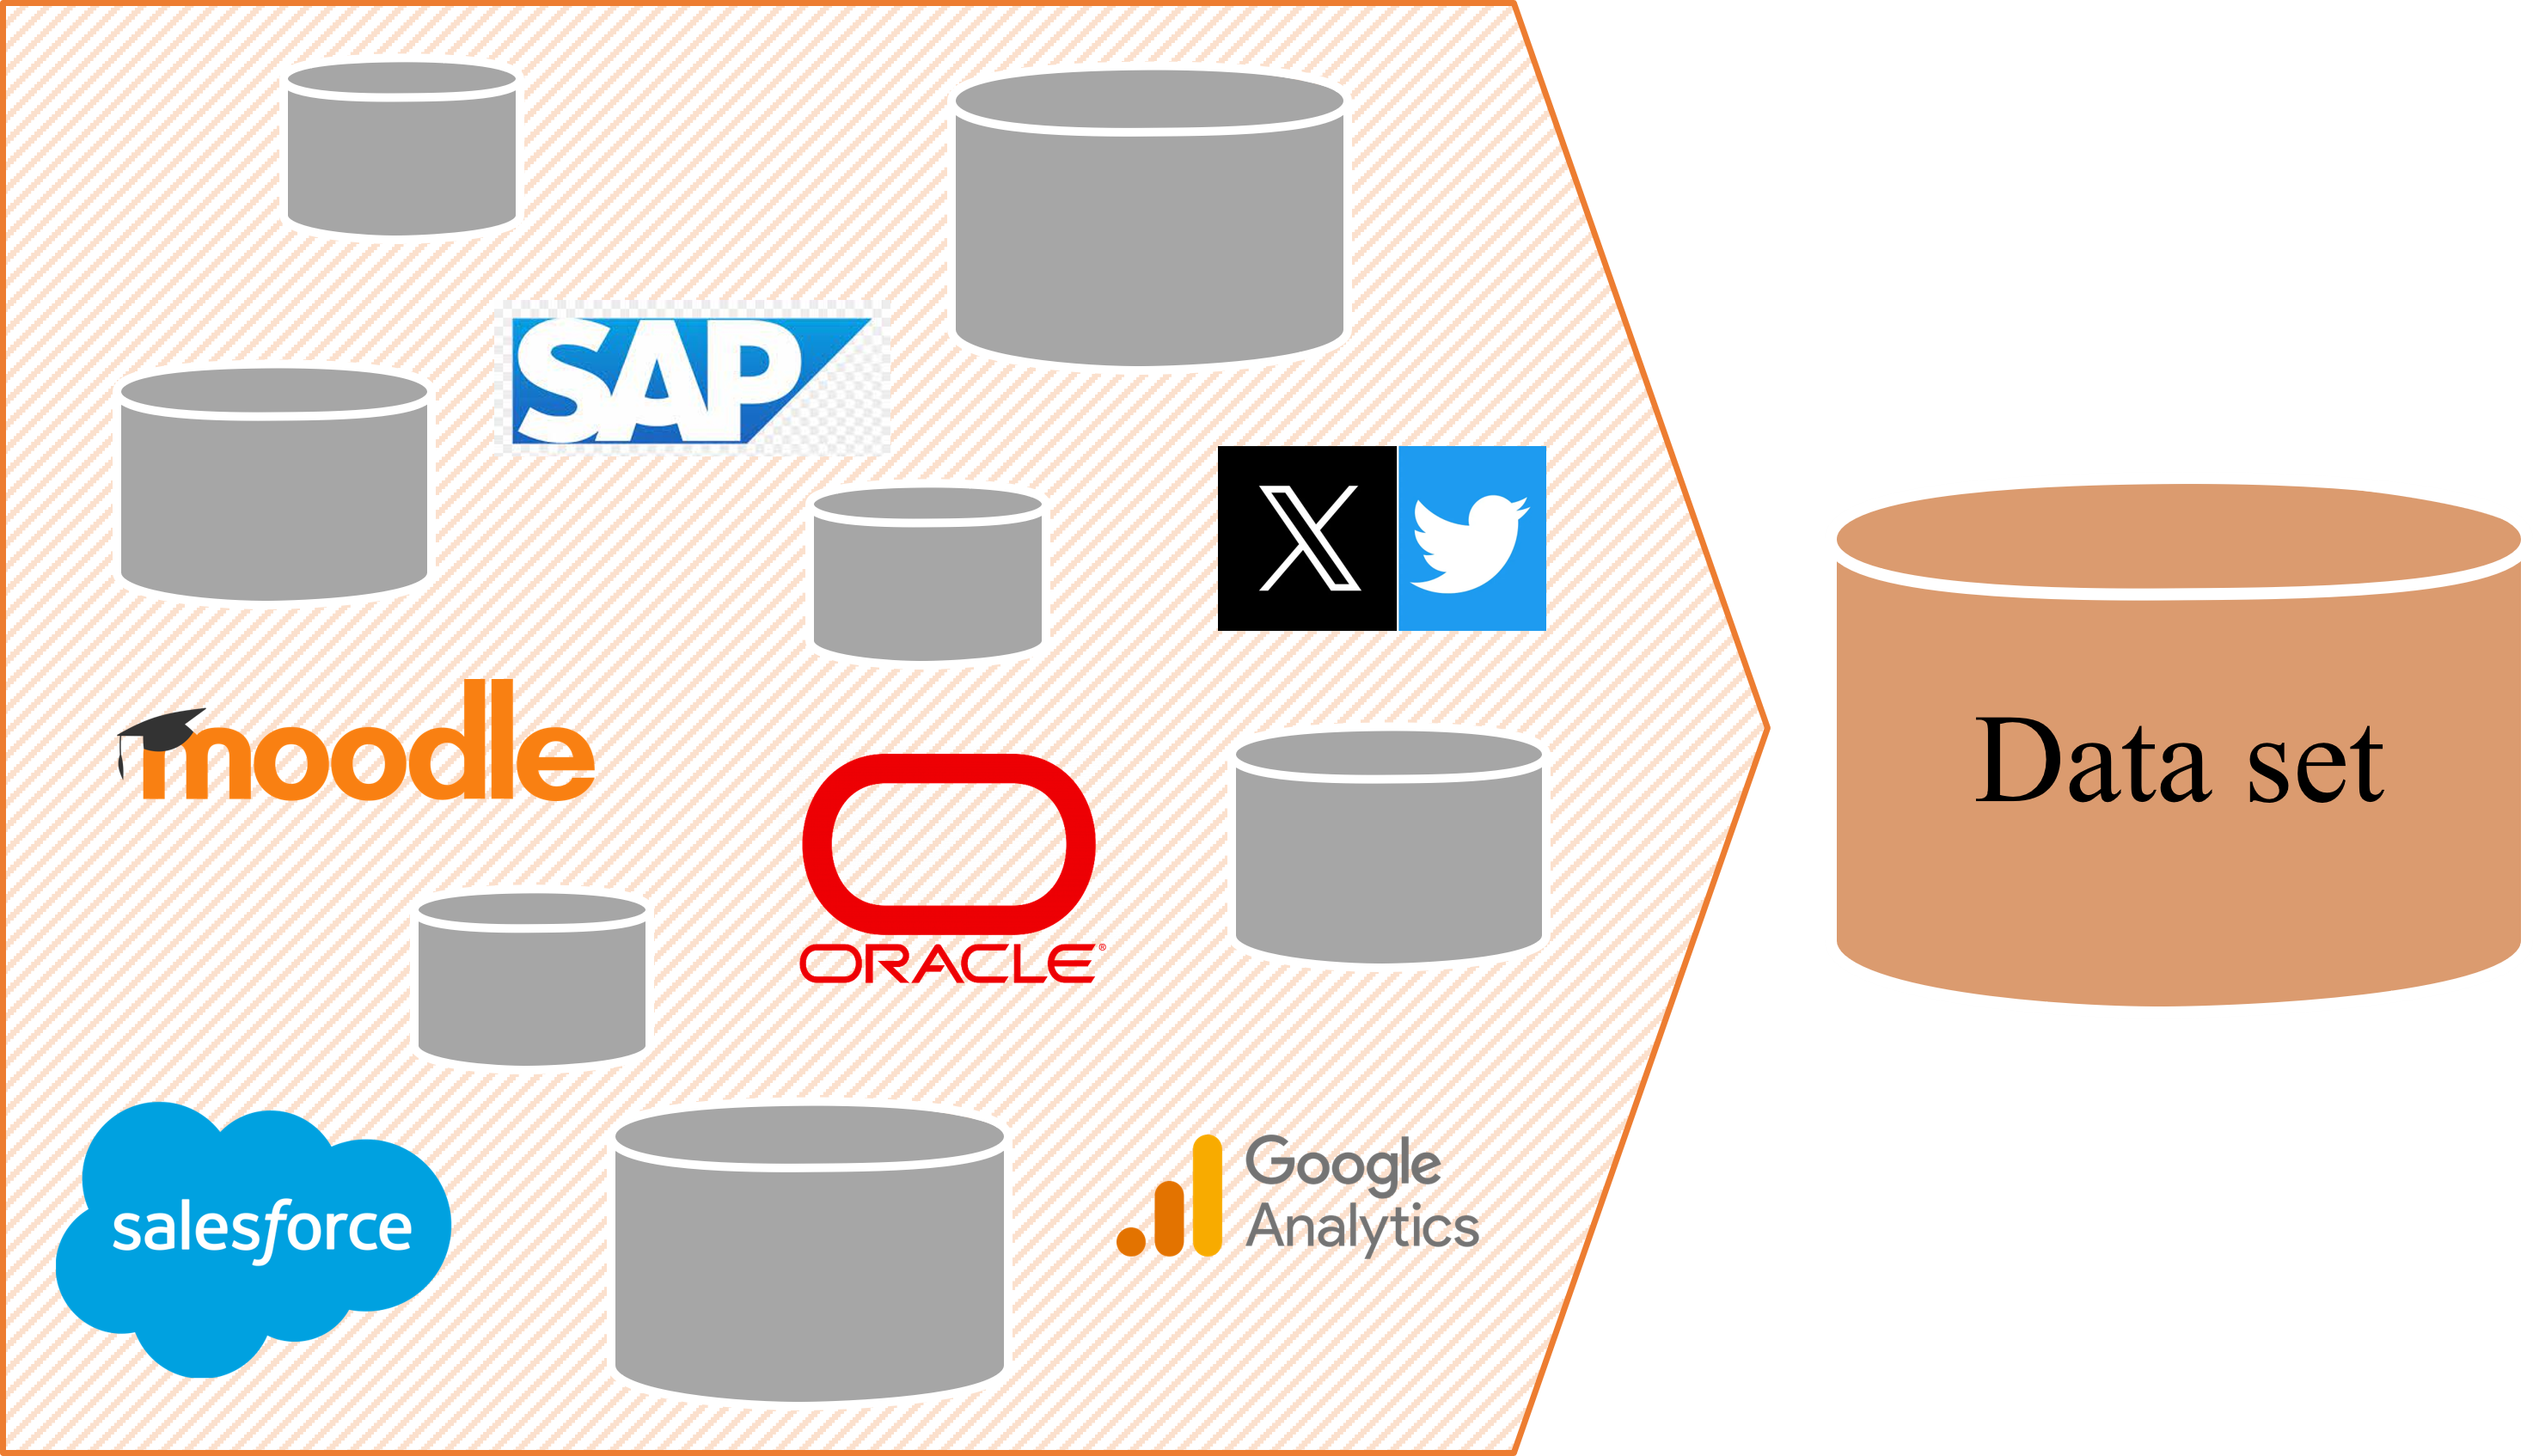
\includegraphics[width=0.4\textwidth]{assets/visualization_and_extraction/data_extraction.png}
  \caption{Data extraction from different sources}
  \label{fig:2_data_extraction}
\end{figure}

The different datatypes were already analyzed in the previous chapter, but still \ref{fig:2_data_types} shows a quick recap. Important to mention, that any unstructured data is considered a bit stream.

\begin{figure}[H]
  \centering
  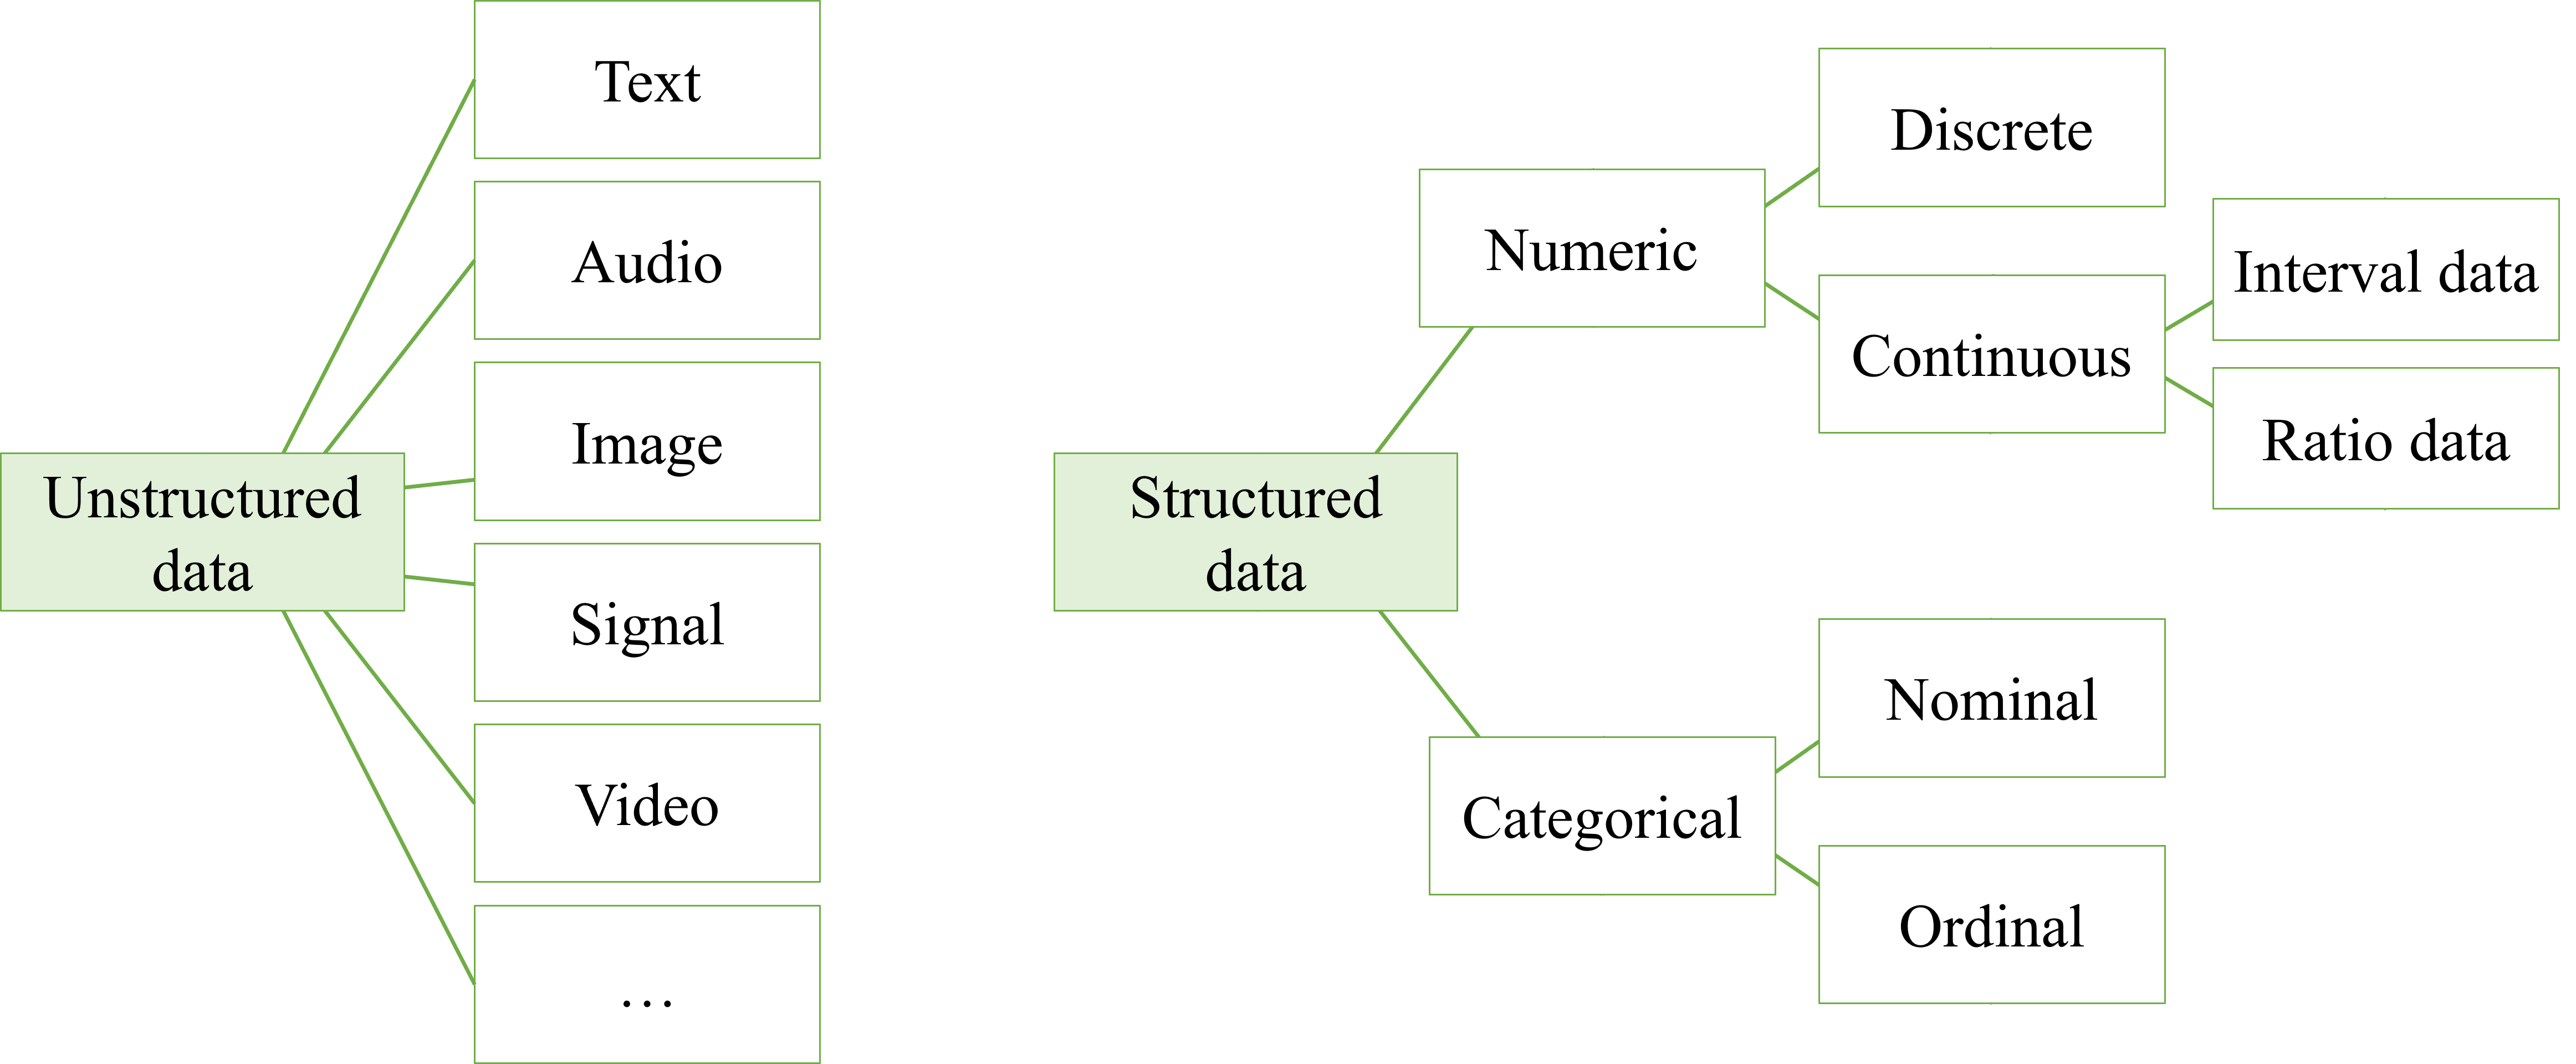
\includegraphics[width=0.7\textwidth]{assets/visualization_and_extraction/data_types.png}
  \caption{Recap: overview types of data}
  \label{fig:2_data_types}
\end{figure}

Important when wanting to obtain any object is of course the feature extraction. The data described by features are usually captured in a tabular form, with rows as the instances and columns as the features. There exist some special features:
\begin{itemize}
  \item \textbf{Time} usually always plays a role in data observation, which is why it is usually one of the recorded features.
  \item Then there are also the \textbf{target features}, in contrast to the descriptive features. The concept was introduced in the last section as part of supervised learning.
\end{itemize}
